\documentclass[12pt,a4paper,titlepage]{article}
\usepackage[utf8]{inputenc}
\usepackage{polski}
\usepackage{graphicx}
\usepackage{xcolor}
\usepackage{minted}
\usepackage{amsmath}
\usepackage{caption}
\usepackage{url}
 
\setminted{
    linenos=true,
    autogobble,
    breaklines,
    frame=lines,
    framerule=1pt,
    framesep=10pt,
    fontsize=\small
}

\setlength{\abovecaptionskip}{0pt}

\newenvironment{longlisting}{}{}
\renewcommand\listingscaption{Code}
 
\DeclareCaptionType{myequation}[][Równanie parametryczne]
\captionsetup[myequation]{labelformat=empty}

\makeatletter
\newcommand{\linia}{\rule{\linewidth}{0.4mm}}
\renewcommand{\maketitle}{\begin{titlepage}
    \vspace*{1cm}
    \begin{center}\small
    Politechnika Wrocławska\\
    Wydział Elektroniki\\
    Grafika Komputerowa i Komunikacja Człowiek-Komputer
    \end{center}
    \vspace{3cm}
    \noindent\linia
    \begin{center}
      \LARGE \textsc{\@title}
         \end{center}
     \linia
    \vspace{0.5cm}
    \begin{flushright}
    \begin{minipage}{7cm}
    \textit{\small Autor:}\\
    \normalsize \textsc{\@author} \par
    \end{minipage}
    \vspace{5cm}

     {\small czwartek, 17\textsuperscript{15}-20\textsuperscript{15} TN}\\
        mgr inż. Szymon Datko
     \end{flushright}
    \vspace*{\stretch{6}}
    \begin{center}
    \@date
    \end{center}
  \end{titlepage}%
}
\makeatother
\author{Justyna Skalska, 225942}
\title{Sprawozdanie z projektu\\
(WebGL)}

\begin{document}
\maketitle
\tableofcontents
\newpage

\section{Omówienie tematu}
Jako projekt na zaliczenie wybrałam webową aplikację z wykorzystaniem WebGL. WebGL pozwala stronom internetowym na wykorzystanie API opartego na OpenGL ES 2.0 do renderowania elementów 2D i 3D w elemencie canvas w przeglądarkach wspierających je bez używania dodatkowych wtyczek. Program WebGL składa się z kodu kontrolującego napisanego w JavaScript i shaderów GLSL (wykonywanych na GPU komputera). Elementy WebGL mogą być łączone z innymi elementami HTML i wkomponowane w inne części strony lub tła. \cite{mozilla} Aplikacja została stworzona przy wykorzystaniu czystego JavaScriptu, CSS oraz HTML5. Pozwala ona na wybranie jednego z trzech obiektów do wizualizacji (sześcian, czworościan, dywan Sierpińskiego). Każda figura ma dodatkowe atrybuty, które można modyfikować.\\
\newline
Sześcian:
\begin{itemize}
    \item tekstura,
    \item rotacja względem 3 osi X,
    \item rotacja względem 3 osi Y,
    \item rotacja względem 3 osi Z.
\end{itemize}
Czworościan:
\begin{itemize}
    \item rotacja względem 3 osi X,
    \item rotacja względem 3 osi Y,
    \item rotacja względem 3 osi Z.
\end{itemize}
Dywan Sierpińskiego:
\begin{itemize}
    \item poziom zniekształcenia,
    \item poziom rekurencji,
    \item rotacja względem 3 osi X,
    \item rotacja względem 3 osi Y,
    \item rotacja względem 3 osi Z.
\end{itemize}
Po wybraniu atrybutów danego obiektu należy je zatwierdzić klikając przycisk "Zatwierdź zmiany". Istnieje także możliwość zatrzymania oraz wznowienia animacji aktualnie wybranej figury.

\section{Omówienie kodu}

\subsection{HTML}

\begin{listing}[H]
\caption{Struktura menu obiektów}
\begin{minted}{html}
<aside class="col s3">
  <div class="figure col s12">
    <div class="row">
      <a class="waves-effect waves-light btn object" onclick="runQube()">Sześcian</a>
      <a class="waves-effect waves-light btn object" onclick="runTetrahedron()">Czworościan</a>
      <a class="waves-effect waves-light btn object" onclick="runSierpinskiCarpet()">Dywan Sierpińskiego</a>
    </div>
  </div>
</aside>
\end{minted}
\end{listing}

\begin{listing}[H]
\caption{Struktura kanwy}
\begin{minted}{html}
<div class="canvas col s12">
  <canvas id="glcanvas" width="700" height="400">
    Brak wsparcia dla elementu HTML5 typu canvas
  </canvas>
  <br>
  <a class="waves-effect waves-light btn" onclick="switchPause(this)">Pauza</a>
  <a class="waves-effect waves-light btn" onclick="apply()">Zatwierdź zmiany</a>
</div>
\end{minted}
\end{listing}

\begin{listing}[H]
\caption{Struktura menu atrybutów}
\begin{minted}{html}
<fieldset class="texture col s12">
  <legend>Wybierz teksturę obiektu:</legend>
  <label>
    <input class="with-gap" type="radio" name="texture" value="1" checked><span>Tekstura 1</span>
  </label>
  <label>
    <input class="with-gap" type="radio" name="texture" value="2"><span>Tekstura 2</span>
  </label>
  <label>
    <input class="with-gap" type="radio" name="texture" value="3"><span>Tekstura 3</span>
  </label>
</fieldset>
<fieldset class="rotate col s12">
  <legend>Wybierz rotację obiektu:</legend>
  <label>
    <input class="filled-in" type="checkbox" id="rotateX">
    <span>Rotacja X</span>
  </label>
  <label>
    <input class="filled-in" type="checkbox" id="rotateY">
    <span>Rotacja Y</span>
  </label>
  <label>
    <input class="filled-in" type="checkbox" id="rotateZ">
    <span>Rotacja Z</span>
  </label>
</fieldset>
<div class="distortion col s6">
  <legend>Wybierz zniekształcenie obiektu:</legend>
  <p class="range-field"><input type="range" name="distortion" min="0" max="100" /></p>
</div>
<div class="level col s6">
  <legend>Wybierz poziom rekurencji obiektu:</legend>
  <p class="range-field"><input type="range" name="level" min="0" max="4" /></p>
</div>
\end{minted}
\end{listing}

\subsection{CSS}
Do ostylowania strony wykorzystano własny plik CSS oraz framework Materialize ze strony \url{https://materializecss.com/} bazujący na stworzonym przez Google Material Design. Wybór padł na CSS zamiast SCSS, ponieważ aplikacja wymaga bardzo mało stylów i wykorzystanie SCSSa oraz Grunta byłoby zbyt czasochłonne na tak małą aplikację.
\begin{longlisting}
\begin{minted}{css}
body {
    padding-top: 25px;
}

span {
    color: black;
}

label {
    margin: 0px 10px 0px 10px;
}

fieldset {
    border: 0;
}

legend {
    padding: 0;
    font-weight: bold;
    margin-bottom: 15px;
}

input[type="range"]:disabled::-webkit-slider-thumb {
    background-color: #949494;
}

input[type="range"]:disabled::-moz-range-thumb {
    background-color: #949494;
}

input[type="range"]:disabled::-ms-thumb {
    background-color: #949494;
}


.object {
    margin: 20px 0px;
    width: 100%;
}

.canvas {
    width: 100%;
    position: relative;
    text-align: center;
}

canvas#glcanvas {
    border: 1px solid #66666D;
    background-color: #545469;
\end{minted}
\end{longlisting}
\begin{listing}
\caption{Arkusz stylów}
\end{listing}

\subsection{JavaScript}
Przy pisaniu kodu zostały wykorzystane fragmenty instrukcji z ćwiczenia o podstawach WebGL ze strony \url{http://www.zsk.ict.pwr.wroc.pl/zsk/dyd/intinz/gk/lab/cw\_8\_dz/}. Nie zostały one w pełni pokazane w sprawozdaniu, ponieważ niektóre fragmenty zostały pominięte, a w ich miejscu znajduje się komentarz. Zamieszczono tylko zmienione oraz nowe fragmenty kodu.

\subsubsection{Funkcje pomocnicze}

\begin{listing}[H]
\caption{Zmienne globalne programu}
\begin{minted}{javascript}
let gl_canvas;
let gl_ctx;

let _position;
let _uv, _color;
let _sampler;

let _triangleVertexBuffer;
let _triangleFacesBuffer;

let _PosMatrix;
let _MovMatrix;
let _ViewMatrix;
let _matrixProjection;
let _matrixMovement;
let _matrixView;
let _cubeTexture;

const rotationSpeed = 0.001;
const zoomRatio = -6;

let X, Y, Z;
let texture;
let animation, pause = false;
let offset, stride, elements;
let figure = 1;

let triangleVertices = [];
let triangleFaces = [];

let vertex = 0;
let recursion = 3;
let distortion = 0;
let length = 4;
\end{minted}
\end{listing}

\begin{listing}[H]
\caption{Funkcje powiązane z inputami}
\begin{minted}{javascript}
function getRotation() {
    X = document.getElementById('rotateX').checked;
    Y = document.getElementById('rotateY').checked;
    Z = document.getElementById('rotateZ').checked;
}

function getTexture() {
    texture = document.querySelector('input[name="texture"]:checked').value;
}

function getDistortion() {
    distortion = document.querySelector('input[name="distortion"]').value;
}

function getRecursion() {
    recursion = document.querySelector('input[name="level"]').value;
}

function disableTextureChoice(isDisabled) {
    document.querySelectorAll('input[name="texture"]').forEach(input => input.disabled = isDisabled);
}

function disableRangeInputs(isDisabled) {
    document.querySelectorAll('input[type="range"]').forEach(input => input.disabled = isDisabled);
}

function switchPause(e) {
    pause = !pause;
    if (pause) {
        e.text = "Start";
    } else {
        e.text = "Pauza";
    }
}
\end{minted}
\end{listing}

\begin{listing}[H]
\caption{Funkcje inicjalizujące WebGL}
\begin{minted}{javascript}
function init() {
    while (triangleVertices.length > 0)
        triangleVertices.pop();
    while (triangleFaces.length > 0)
        triangleFaces.pop();
    
    gl_canvas = document.getElementById("glcanvas");
    gl_ctx = gl_getContext(gl_canvas);
}

// funkcja główna 
function runWebGL() {
    getRotation();    
    gl_initBuffers();
    gl_setMatrix();
    gl_draw();
}

// pobranie kontekstu WebGL
function gl_getContext(canvas) {
    try {
        var ctx = canvas.getContext("webgl");
        ctx.viewportWidth = canvas.width;
        ctx.viewportHeight = canvas.height;
    } catch (e) {}
    if (!ctx) {
        document.write('Nieudana inicjalizacja kontekstu WebGL.')
    }
    return ctx;
}
\end{minted}
\end{listing}


\subsubsection{Sześcian}

\begin{listing}[H]
\caption{Funkcja zwracająca dane wierzchołków sześcianu}
\begin{minted}{javascript}
function getQubeTriangleVertices() {
    return [
        -1, -1, -1, 0, 0,
        1, -1, -1, 1, 0,
        1, 1, -1, 1, 1,
        -1, 1, -1, 0, 1,
        -1, -1, 1, 0, 0,
        1, -1, 1, 1, 0,
        1, 1, 1, 1, 1,
        -1, 1, 1, 0, 1,
        -1, -1, -1, 0, 0,
        -1, 1, -1, 1, 0,
        -1, 1, 1, 1, 1,
        -1, -1, 1, 0, 1,
        1, -1, -1, 0, 0,
        1, 1, -1, 1, 0,
        1, 1, 1, 1, 1,
        1, -1, 1, 0, 1,
        -1, -1, -1, 0, 0,
        -1, -1, 1, 1, 0,
        1, -1, 1, 1, 1,
        1, -1, -1, 0, 1,
        -1, 1, -1, 0, 0,
        -1, 1, 1, 1, 0,
        1, 1, 1, 1, 1,
        1, 1, -1, 0, 1
    ];
}
\end{minted}
\end{listing}

\begin{listing}[H]
\caption{Funkcja zwracająca dane ścian sześcianu}
\begin{minted}{javascript}
function getQubeTriangleFaces() {
    return [
        0, 1, 2,
        0, 2, 3,
        4, 5, 6,
        4, 6, 7,
        8, 9, 10,
        8, 10, 11,
        12, 13, 14,
        12, 14, 15,
        16, 17, 18,
        16, 18, 19,
        20, 21, 22,
        20, 22, 23
    ];
}
\end{minted}
\end{listing}

\begin{listing}[H]
\caption{Inicjalizacja zmiennych sześcianu}
\begin{minted}{javascript}
triangleVertices = getTetrahedronTriangleVertices();
triangleFaces = getTetrahedronTriangleFaces();
stride = (2 + 3) * Float32Array.BYTES_PER_ELEMENT;
offset = 3 * Float32Array.BYTES_PER_ELEMENT;
elements = 4 * 3;
\end{minted}
\end{listing}

\begin{listing}[H]
\caption{Funkcja rysująca sześcian}
\begin{minted}{javascript}
function runQube() {
    figure = 1;
    disableTextureChoice(false);
    disableRangeInputs(true);

    init();
    getTexture();
    gl_initShaders();
    _cubeTexture = gl_initTexture();
    
    runWebGL();
}
\end{minted}
\end{listing}

\subsubsection{Czworościan}

\begin{listing}[H]
\caption{Funkcja zwracająca dane wierzchołków czworościanu}
\begin{minted}{javascript}
function getTetrahedronTriangleVertices() {
    return [
        0, 2, -1, 1, 1,
        -2, -1, -1, 0, 0,
        2, -1, -1, 0, 1,
        0, 0, 2, 1, 0
    ];
}
\end{minted}
\end{listing}

\begin{listing}[H]
\caption{Funkcja zwracająca dane ścian czworościanu}
\begin{minted}{javascript}
function getTetrahedronTriangleFaces() {
    return [
        0, 1, 2,
        0, 2, 3,
        0, 3, 1,
        2, 1, 3
    ];
}
\end{minted}
\end{listing}

\begin{listing}[H]
\caption{Inicjalizacja zmiennych czworościanu}
\begin{minted}{javascript}
triangleVertices = getQubeTriangleVertices();
triangleFaces = getQubeTriangleFaces();
stride = (2 + 3) * Float32Array.BYTES_PER_ELEMENT;
offset = 3 * Float32Array.BYTES_PER_ELEMENT;
elements = 5 * 3 * 2;
\end{minted}
\end{listing}

\begin{listing}[H]
\caption{Funkcja rysująca czworościan}
\begin{minted}{javascript}
function runTetrahedron() {
    figure = 2;
    disableTextureChoice(true);
    disableRangeInputs(true);

    init();
    getTexture();
    gl_initShaders();
    _cubeTexture = gl_initTexture();
    
    runWebGL();
}
\end{minted}
\end{listing}

\subsubsection{Dywan Sierpińskiego}

\begin{listing}[H]
\caption{Funkcja dodająca wierzchołki dywanu}
\begin{minted}{javascript}
function addVertex(x, y, variation) {
    triangleVertices.push(x + variation);
    triangleVertices.push(y + variation);
    // losowy kolor wierzchołka
    triangleVertices.push(Math.random());
    triangleVertices.push(Math.random());
    triangleVertices.push(Math.random());
}
\end{minted}
\end{listing}



\begin{listing}[H]
\caption{Funkcja dodająca ściany dywanu Sierpińskiego}
\begin{minted}{javascript}
function addFace(vertex) {
    // pierwsza połowa kwadratu (prawy dolny trójkąt)
    triangleFaces.push(vertex - 3);
    triangleFaces.push(vertex - 2);
    triangleFaces.push(vertex - 1);

    // druga połowa kwadratu (lewy górny trójkąt)
    triangleFaces.push(vertex - 3);
    triangleFaces.push(vertex - 1);
    triangleFaces.push(vertex);

    elements += 6; // powiększenie ilości elementów bufora indeksów
}
\end{minted}
\end{listing}

\begin{listing}[H]
\caption{Funkcja zwracająca odchylenie punktu dywanu Sierpińskiego}
\begin{minted}{javascript}
function getVariation(length) {
        // wyliczenie właściwego przesunięcia deformacji
        let variation;
        if (distortion !== 0) {
            variation = (Math.random() % (0.1 * length)) * (distortion * 0.1);
        } else {
            variation = 0;
        }
        
        // zapewnienie, że przesunięcie w lewo i prawo występują z takim samym prawdopodobieństwem
        let probability = Math.random();
        if (probability < 0.5) {
            variation = -variation;
        }

        return variation
}
\end{minted}
\end{listing}

\begin{listing}[H]
\caption{Funkcja rysująca dywan Sierpińskiego}
\begin{minted}{javascript}
function drawSierpinskiCarpet(x, y, length, level) {
    if (level > 0) {
        length = length / 3;
        level -= 1;
        drawSierpinskiCarpet(x - (2 * length), y, length, level);
        drawSierpinskiCarpet(x - length, y, length, level);
        drawSierpinskiCarpet(x, y, length, level);

        drawSierpinskiCarpet(x - (2 * length), y - length, length, level);
        drawSierpinskiCarpet(x, y - length, length, level);

        drawSierpinskiCarpet(x - (2 * length), y - (2 * length), length, level);
        drawSierpinskiCarpet(x - length, y - (2 * length), length, level);
        drawSierpinskiCarpet(x, y - (2 * length), length, level);
    } else {
        let variation = getVariation(length);
        // prawy górny wierzchołek kwadratu
        addVertex(x, y, variation);
        if (vertex !== 0)
            vertex = vertex + 1;

        // prawy dolny wierzchołek kwadratu
        addVertex(x, y - length, variation);
        vertex = vertex + 1;

        // lewy dolny wierzchołek kwadratu
        addVertex(x - length, y -length, variation);
        vertex = vertex + 1;

        // lewy górny wierzchołek kwadratu
        addVertex(x - length, y, variation);
        vertex = vertex + 1;

        addFace(vertex);
    }
}
\end{minted}
\end{listing}

\begin{listing}[H]
\caption{Inicjalizacja zmiennych dywanu Sierpińskiego}
\begin{minted}{javascript}
stride = (2 + 3) * Float32Array.BYTES_PER_ELEMENT;
offset = 2 * Float32Array.BYTES_PER_ELEMENT;
\end{minted}
\end{listing}

\begin{longlisting}
\begin{minted}{javascript}
function gl_draw() {
    if (animation) {
        // anuluje wykonywanie kodu animacji
        window.cancelAnimationFrame(animation)
    }

    ... // fragment bez zmiany względem kodu z instrukcji

    const animate = function (time) {
        if (!pause) {
            const dAngle = rotationSpeed * (time - timeOld);
            if (X) {
                MATRIX.rotateX(_matrixMovement, dAngle);
            }
            if (Y) {
                MATRIX.rotateY(_matrixMovement, dAngle);
            }
            if (Z) {
                MATRIX.rotateZ(_matrixMovement, dAngle);
            }
        }

        timeOld = time;

        ... // fragment bez zmiany względem kodu z instrukcji

        if (figure === 3) {
            // figura 2D z kolorem
            gl_ctx.vertexAttribPointer(_position, 2, gl_ctx.FLOAT, false, stride, 0);
            gl_ctx.vertexAttribPointer(_color, 3, gl_ctx.FLOAT, false, stride, offset);
        } else {
            if (_cubeTexture.webglTexture) {
                gl_ctx.activeTexture(gl_ctx.TEXTURE0);
                gl_ctx.bindTexture(gl_ctx.TEXTURE_2D, _cubeTexture.webglTexture);
            }
            // figura 3D z teksturą
            gl_ctx.vertexAttribPointer(_position, 3, gl_ctx.FLOAT, false, stride, 0);
            gl_ctx.vertexAttribPointer(_uv, 2, gl_ctx.FLOAT, false, stride, offset);
        }

        gl_ctx.bindBuffer(gl_ctx.ARRAY_BUFFER, _triangleVertexBuffer);
        gl_ctx.bindBuffer(gl_ctx.ELEMENT_ARRAY_BUFFER, _triangleFacesBuffer);

        gl_ctx.drawElements(gl_ctx.TRIANGLES, elements, gl_ctx.UNSIGNED_SHORT, 0);
        gl_ctx.flush();

        // wykonaj kod po następnym odświeżeniu ekranu
        animation = window.requestAnimationFrame(animate);
    };

    animate(0);
}
\end{minted}
\end{longlisting}
\begin{listing}
\caption{Funkcja rysująca}
\end{listing}

\begin{listing}[H]
\caption{Funkcja rysująca dywanu Sierpińskiego}
\begin{minted}{javascript}
function runSierpinskiCarpet() {
    figure = 3;
    disableTextureChoice(true);
    disableRangeInputs(false);

    elements = 0;
    vertex = 0;
    init();
    getDistortion();
    getRecursion();
    gl_initShadersForSierpinskiCarpet();
    drawSierpinskiCarpet(length / 2, length / 2, length, recursion);
    
    runWebGL();
}
\end{minted}
\end{listing}

\newpage
\section{Rezultat prac}
Skończony projekt znajduje się pod adresem \url{https://jastka4.github.io/GKiKC-K-project}.

\subsection{Sześcian}
\begin{figure}[H]
\centering
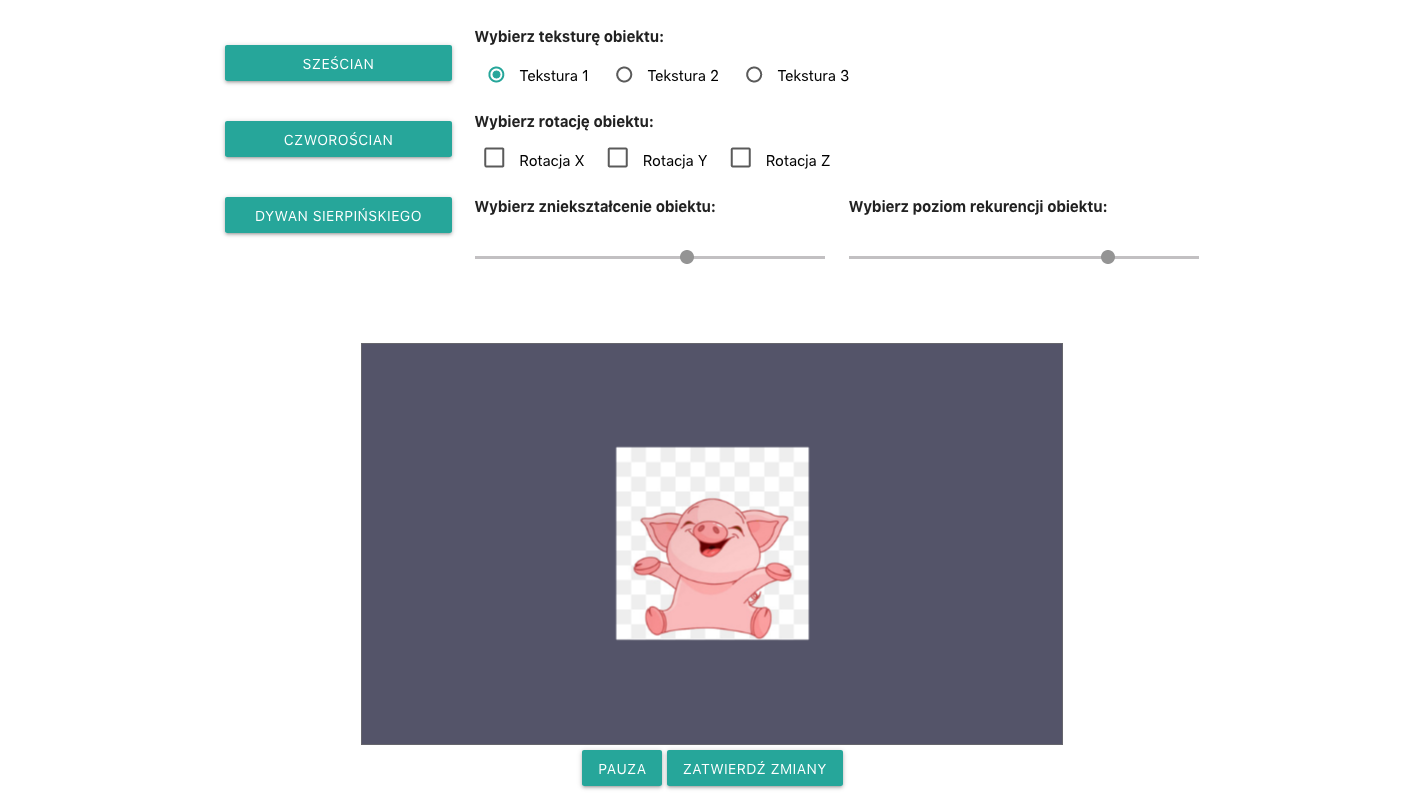
\includegraphics[width=14cm]{images/qube_still.png}
\caption{Sześcian z nałożoną teksturą}
\label{fig:eggWithLight}
\end{figure}

\begin{figure}[H]
\centering
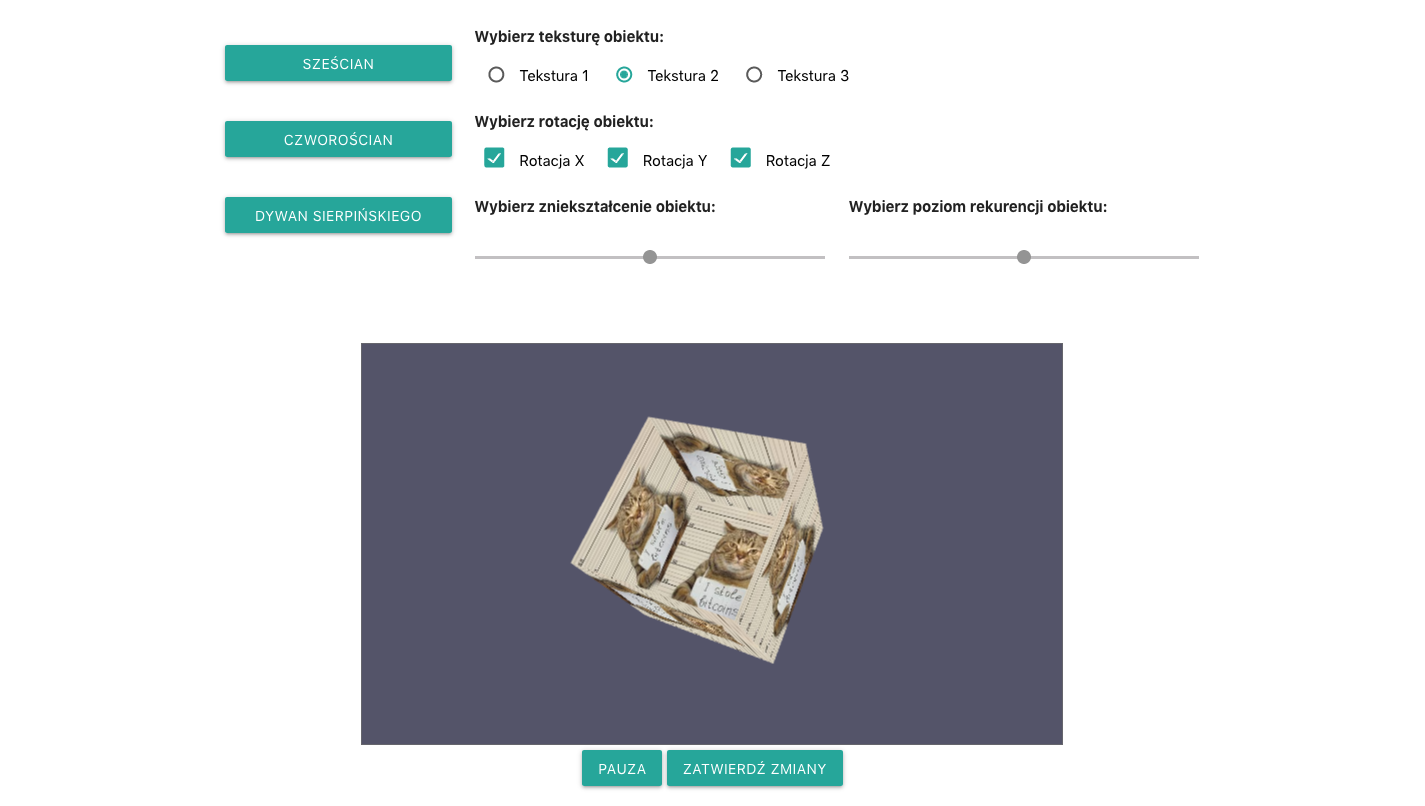
\includegraphics[width=14cm]{images/qube_rotating.png}
\caption{Sześcian z nałożoną teksturą podczas obrotu}
\label{fig:eggWithLight}
\end{figure}

\subsection{Czworościan}
\begin{figure}[H]
\centering
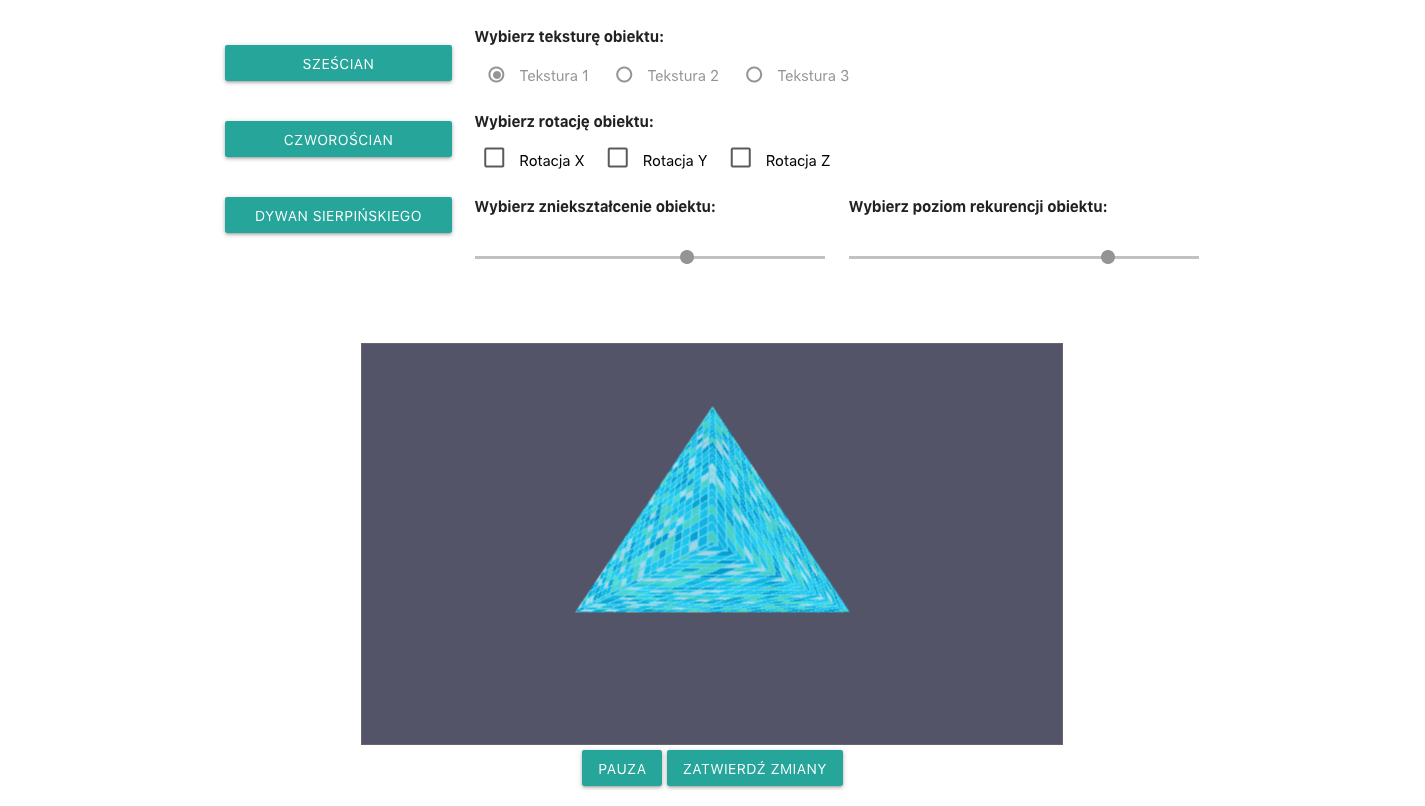
\includegraphics[width=14cm]{images/tetrahedron_still.png}
\caption{Czworościan z nałożoną teksturą}
\label{fig:eggWithLight}
\end{figure}

\begin{figure}[H]
\centering
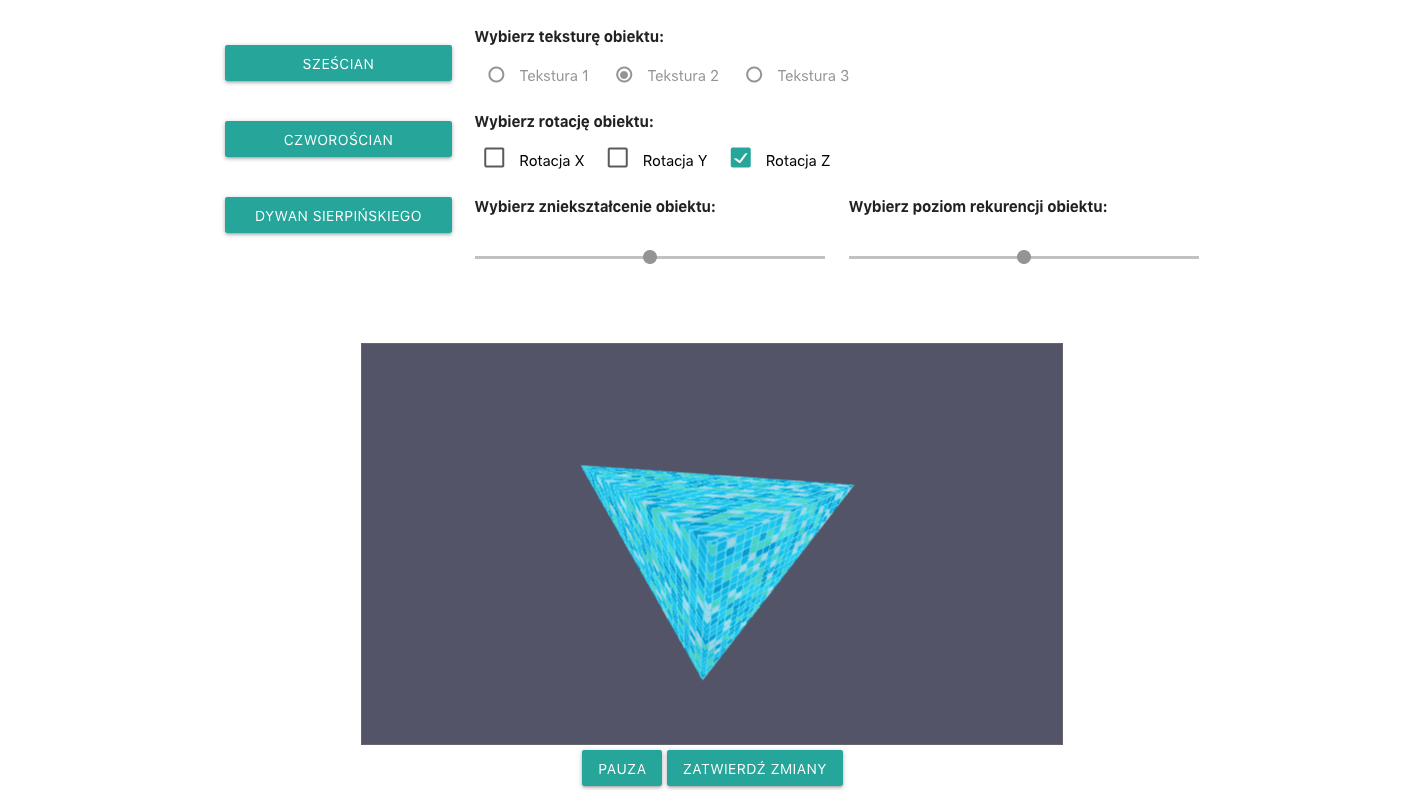
\includegraphics[width=14cm]{images/tetrahedron_rotating.png}
\caption{Czworościan z nałożoną teksturą podczas obrotu}
\label{fig:eggWithLight}
\end{figure}

\subsection{Dywan Sierpińskiego}
\begin{figure}[H]
\centering
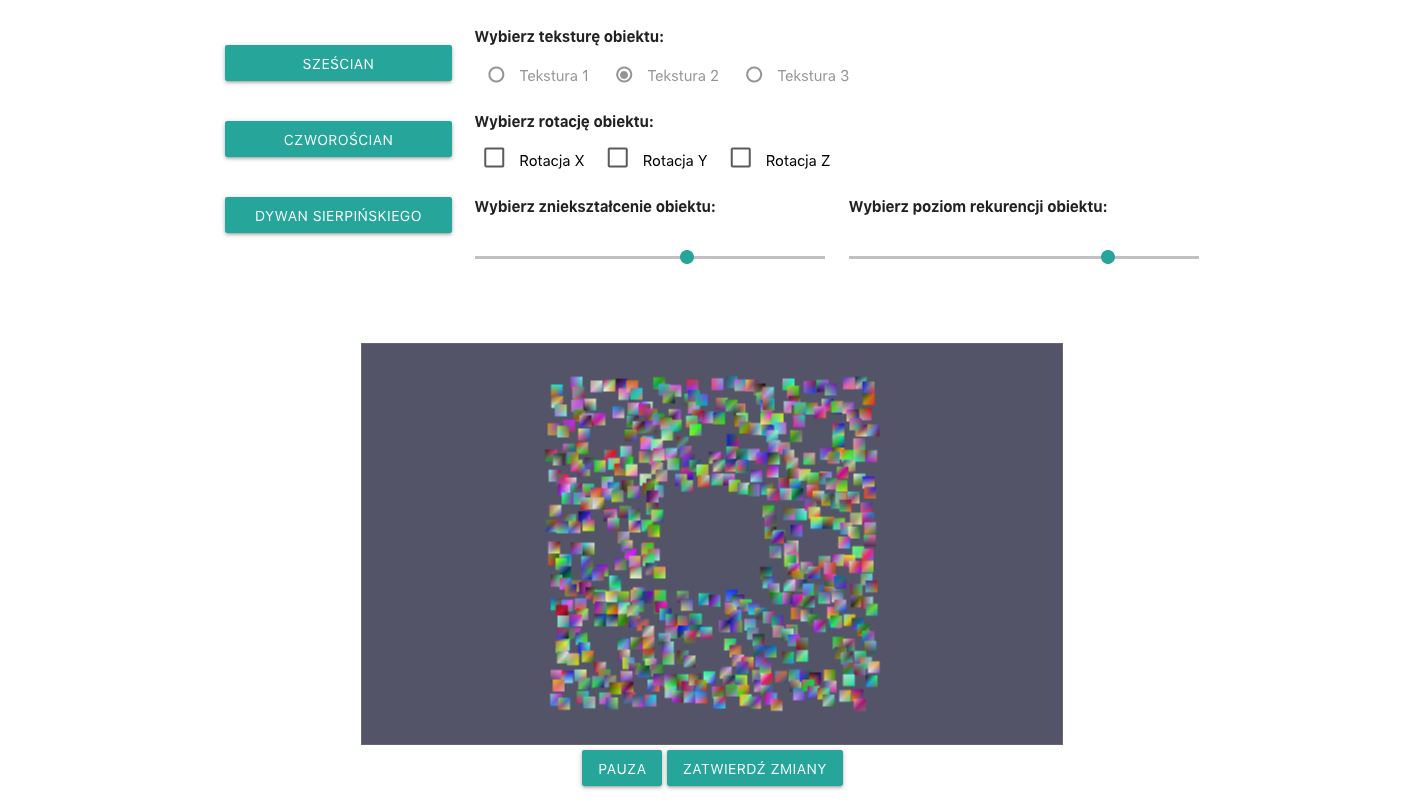
\includegraphics[width=14cm]{images/carpet_still.png}
\caption{Dywan Sierpińskiego z deformacjami}
\label{fig:eggWithLight}
\end{figure}

\begin{figure}[H]
\centering
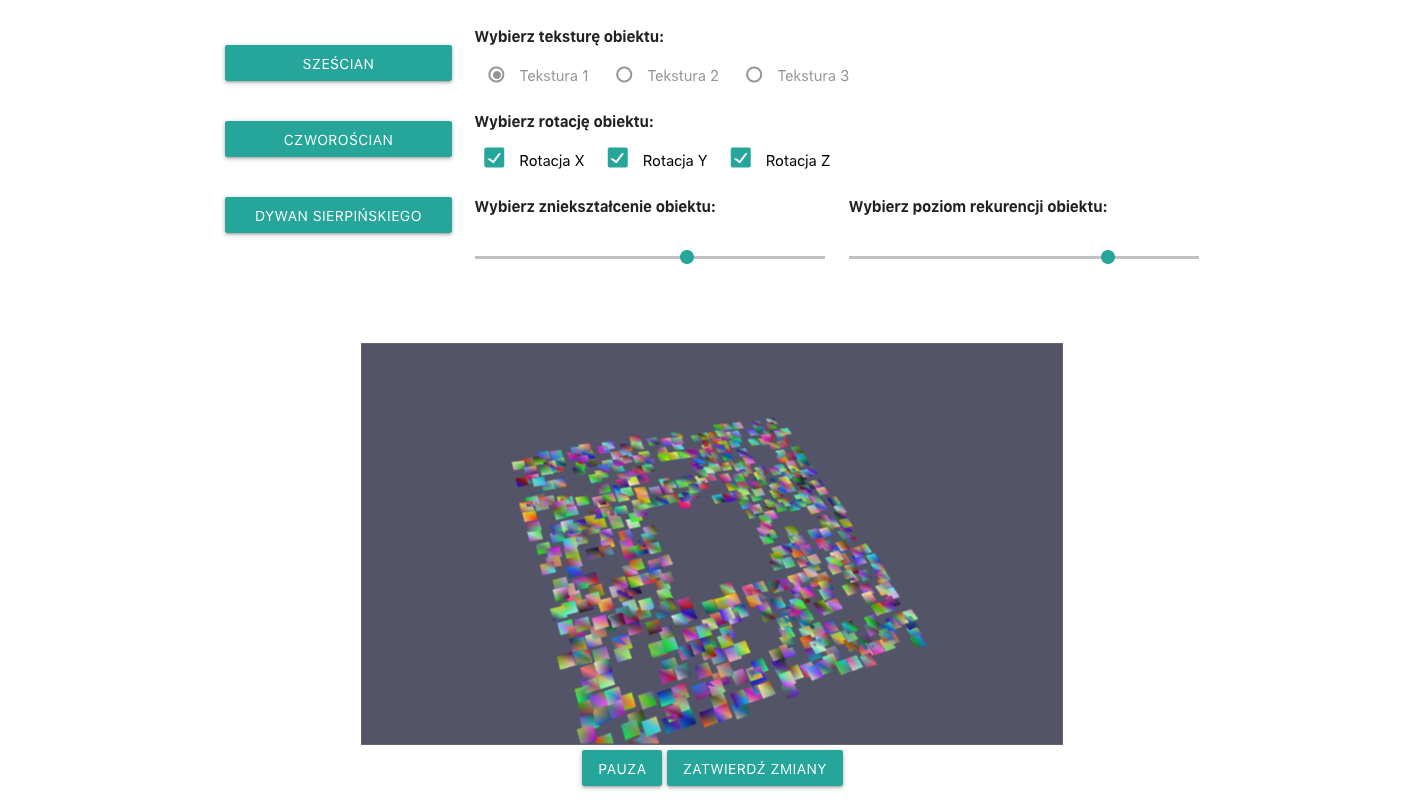
\includegraphics[width=14cm]{images/carpet_rotating.png}
\caption{Dywan Sierpińskiego z deformacjami podczas obrotu}
\label{fig:eggWithLight}
\end{figure}

\begin{figure}[H]
\centering
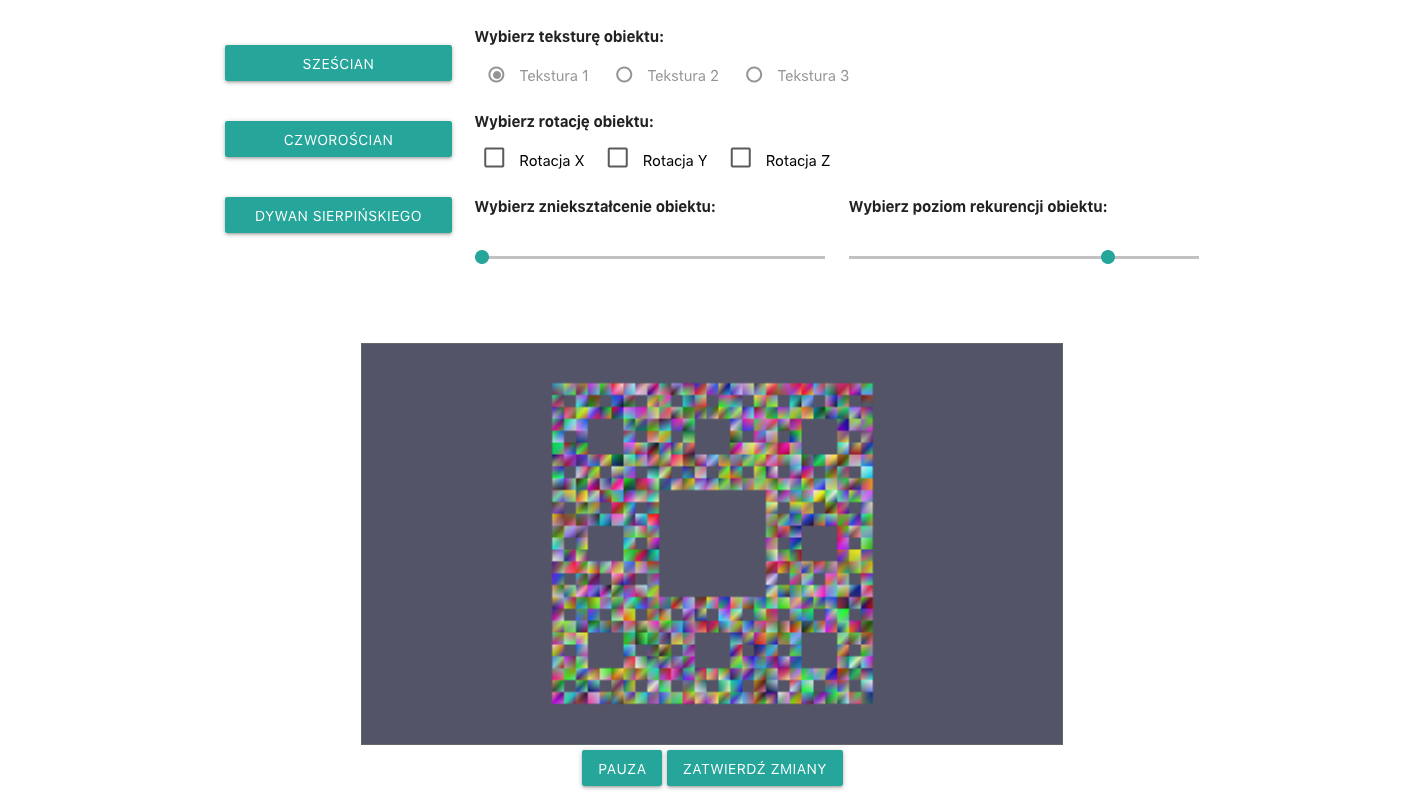
\includegraphics[width=14cm]{images/carpet_still_no_disruption.png}
\caption{Dywan Sierpińskiego bez deformacji}
\label{fig:eggWithLight}
\end{figure}

\begin{figure}[H]
\centering
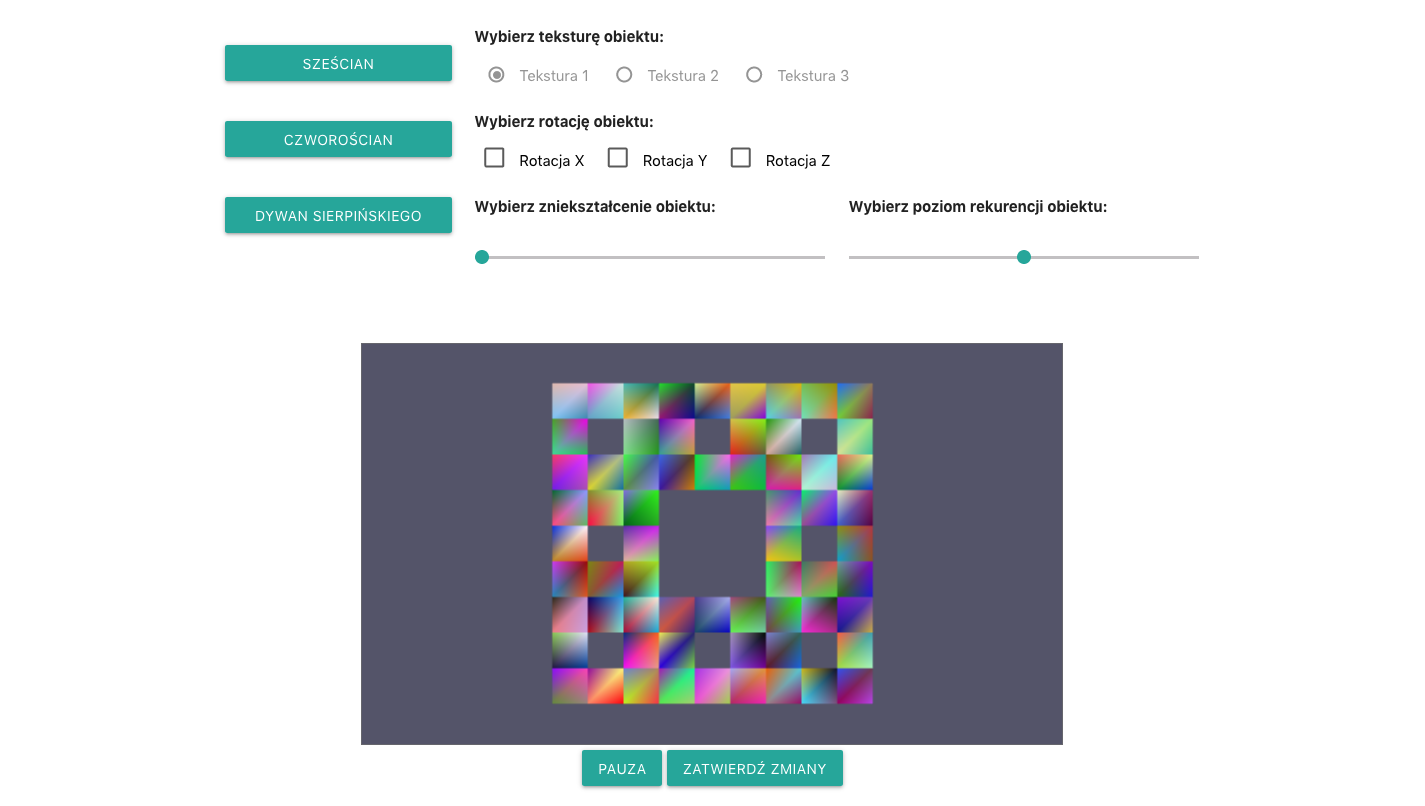
\includegraphics[width=14cm]{images/carpet_still_no_disruption_smaller_level.png}
\caption{Dywan Sierpińskiego z bez deformacji (mniejsza rekurencja)}
\label{fig:eggWithLight}
\end{figure}

\section{Wnioski}
Podczas wykonywania tego zadania udało mi się zapoznać z podstawami WebGL. Różni się on nieco od wcześniej poznanego OpenGLa, ponieważ jest on oparty na OpenGL ES. Dzięki temu projektowi w przyszłości będzie mi łatwiej wykonać ciekawe projekty webowe z wykorzystaniem grafiki 3D.
\newpage

\bibliographystyle{unsrt}
\bibliography{references}
\listoffigures
\listoflistings
\end{document}
